\section{ФОРМУЛЫ ВЕЛИЧИН}

Все формулы применяются для выборки из генеральной совокупности
$\vec X = \big( x_1, \dots, x_n \big)$.

Максимальное значение выборки вычисляется по формуле \ref{eq:max}.

\begin{equation}\label{eq:max}
    M_{\max} = \max \{ x_1, \dots, x_n \}
\end{equation}

Минимальное значение выборки вычисляется по формуле \ref{eq:min}.

\begin{equation}\label{eq:min}
    M_{\min} = \min \{ x_1, \dots, x_n \}
\end{equation}

Размах выборки вычисляется по формуле \ref{eq:r}.

\begin{equation}\label{eq:r}
    R = M_{\max} - M_{\min}
\end{equation}

Оценка математического ожидания вычисляется по формуле \ref{eq:mu}.

\begin{equation}\label{eq:mu}
    \hat \mu = \overline x = \frac{1}{n} \sum_{i=1}^{n} x_i
\end{equation}

Оценка дисперсии вычисляется по формуле \ref{eq:s}.

\begin{equation}\label{eq:s}
    S^2 = \frac{1}{n-1} \sum_{i=1}^n (x_i - \overline{x})^2
\end{equation}

\section{ЭМПИРИЧЕСКАЯ ПЛОТНОСТЬ И ГИСТОГРАММА}

\textbf{Эмпирической плотностью}
(отвечающей выборке $\vec x$) называют функцию

\begin{equation*}
    \hat f_n(x) =
    \begin{cases}
        \frac{n_i}{n \Delta}, x \in J_i, i = \overline{1; p} \\
        0, \text{ иначе} \\
    \end{cases}
\end{equation*}

\textbf{Гистограммой} называют график эмпирической плотности.

\section{ЭМПИРИЧЕСКАЯ ФУНКЦИЯ РАСПРЕДЕЛЕНИЯ}

\textbf{Эмпирической функцией распределения} называют функцию

\begin{equation*}
    F_n : \mathcal R \to \mathcal R
\end{equation*}

определенную условием

\begin{equation*}
    F_n(x) = \frac{n(x, \vec x)}{n}
\end{equation*}

\section{ТЕКСТ ПРОГРАММЫ}

\begin{lstlisting}[caption=Точка входа в программу]
function lab1()
    X = [
        -7.50, -6.61, -7.85, -7.72, -8.96, ...
        -6.55, -7.82, -6.55, -6.87, -5.95, ...
        -5.05, -4.56, -6.14, -6.83, -6.33, ...
        -7.67, -4.65, -6.30, -8.01, -5.88, ...
        -5.38, -7.06, -6.85, -5.53, -7.83, ...
        -5.89, -7.57, -6.76, -6.02, -4.62, ...
        -8.55, -6.37, -7.52, -5.78, -6.12, ...
        -8.82, -5.14, -7.68, -6.14, -6.48, ...
        -7.14, -6.25, -7.32, -5.51, -6.97, ...
        -7.86, -7.04, -6.24, -6.41, -6.00, ...
        -7.46, -6.00, -6.06, -5.94, -5.39, ...
        -5.06, -6.91, -8.06, -7.24, -6.42, ...
        -8.73, -6.20, -7.35, -5.90, -5.02, ...
        -5.93, -7.56, -7.49, -6.26, -6.06, ...
        -7.35, -5.10, -6.52, -7.97, -5.71, ...
        -7.62, -7.33, -5.31, -6.21, -7.28, ...
        -7.99, -4.65, -7.07, -7.31, -7.72, ...
        -5.22, -7.00, -7.17, -6.64, -7.00, ...
        -6.12, -6.57, -6.07, -6.65, -7.60, ...
        -6.92, -6.78, -6.85, -7.90, -7.40, ...
        -5.32, -6.58, -6.71, -5.07, -5.80, ...
        -4.87, -5.90, -7.43, -7.03, -6.67, ...
        -7.72, -5.83, -7.49, -6.68, -6.71, ...
        -7.31, -7.83, -7.92, -5.97, -6.34, ...
    ];

    Params(X);
    Intervals(X);
    MakeGraphs(X);
end
\end{lstlisting}

\begin{lstlisting}[caption=Функция для вычисления параметров]
% Подсчет параметров выборки и вывода их на экран
% [in] X - генеральная совокупность
function Params(X)
    % Максимальное значение выборки
    maxX = max(X);
    fprintf("Mmax = %.3f\n", maxX);

    % Минимальное значение выборки
    minX = min(X);
    fprintf("Mmin = %.3f\n", minX);

    % Разброс выборки
    R = maxX - minX;
    fprintf("R    = %.3f\n", R);

    % Оценка математического ожидания выборки
    M = mean(X);
    fprintf("M    = %.3f\n", M);

    % Оценка дисперсии выборки
    D = FindD(X);
    fprintf("D    = %.3f\n", D);
end

% Функция для вычисления оценки дисперсии выборки
% [in] X - генеральная совокупность
% [return] оценка дисперсии выборки
function D = FindD(X)
    D = sum((X - mean(X)) .^ 2) / (length(X) - 1);
    return
end
\end{lstlisting}

\begin{lstlisting}[caption=Вычисление интервалов]
% Функция для группировки значений в m интервалов
% и вывода на экран количества элементов в каждом интервале
% (m = [log2(n)] + 2)
% [in] X - генеральная совокупность
function Intervals(X)
    m = floor(log2(length(X))) + 2;
    delta = (max(X) - min(X)) / m;
    borders = min(X) : delta : max(X);

    fprintf('\n%d intervals:\n', m);
    for i = 1:(length(borders) - 1)
        count = 0;
        for x = X
            % Последний интевал включает в себя правое значение
            if (i == length(borders) - 1) && (x >= borders(i)) && ...
               (x <= borders(i + 1))
                count = count + 1;
            % Остальные интервалы включительно только слева
            elseif (x >= borders(i)) && (x < borders(i + 1))
                count = count + 1;
            end
        end

        printableString = '[%.3f; %.3f) -> %d\n';
        if (i == length(borders) - 1)
            printableString = '[%.3f; %.3f] -> %d\n';
        end

        fprintf(printableString, borders(i), borders(i + 1), count);
    end
end
\end{lstlisting}

\begin{lstlisting}[caption=Рисование графиков]
% Функция для рисования графиков
% [in] X - генеральная совокупность
function MakeGraphs(X)
    x = sort(X);

    subplot(2, 1, 1);
    % Гистограмма
    histogram(X, 'Normalization', 'pdf');
    hold on;
    % График функции плотности распределения нормальной случайной величины
    f = normpdf(x, mean(x), sqrt(FindD(x)));
    p1 = plot(x, f);
    p1.LineWidth = 2;
    hold off;
    legend({'Гистограмма', 'Функция плотности распределения'}, ...
        'Location','northwest');

    subplot(2, 1, 2);
    % Эмперическая функция распределения
    histogram(X, 'Normalization', 'cdf');
    hold on;
    % Функция распределения нормальной случайной величины
    f = normcdf(x, mean(x), sqrt(FindD(x)));
    p2 = plot(x, f);
    p2.LineWidth = 2;
    hold off;
    legend({'Эмперическая функция распределения', ...
        'Функция распределения'}, ...
        'Location','northwest');
end
\end{lstlisting}

\section{РЕЗУЛЬТАТЫ РАСЧЕТОВ}

\begin{equation*}
    M_{\max} = -4.560
\end{equation*}

\begin{equation*}
    M_{\min} = -8.960
\end{equation*}

\begin{equation*}
    R = 4.400
\end{equation*}

\begin{equation*}
    \hat \mu = -6.649
\end{equation*}

\begin{equation*}
    S^2 = 0.948
\end{equation*}

\setlength\extrarowheight{4pt}
\begin{table}[H]
    \centering
    \begin{tabular}{|c|c|}
        \hline
        $[-8.960; -8.410)$ & 4 \\
        \hline
        $[-8.410; -7.860)$ & 6 \\
        \hline
        $[-7.860; -7.310)$ & 25 \\
        \hline
        $[-7.310; -6.760)$ & 20 \\
        \hline
        $[-6.760; -6.210)$ & 23 \\
        \hline
        $[-6.210; -5.660)$ & 24 \\
        \hline
        $[-5.660; -5.110)$ & 8 \\
        \hline
        $[-5.110; -4.560]$ & 10 \\
        \hline
    \end{tabular}
    \caption{Группировка значений выборки в 8 интервалов}
\end{table}

\begin{figure}[H]
    \centering
    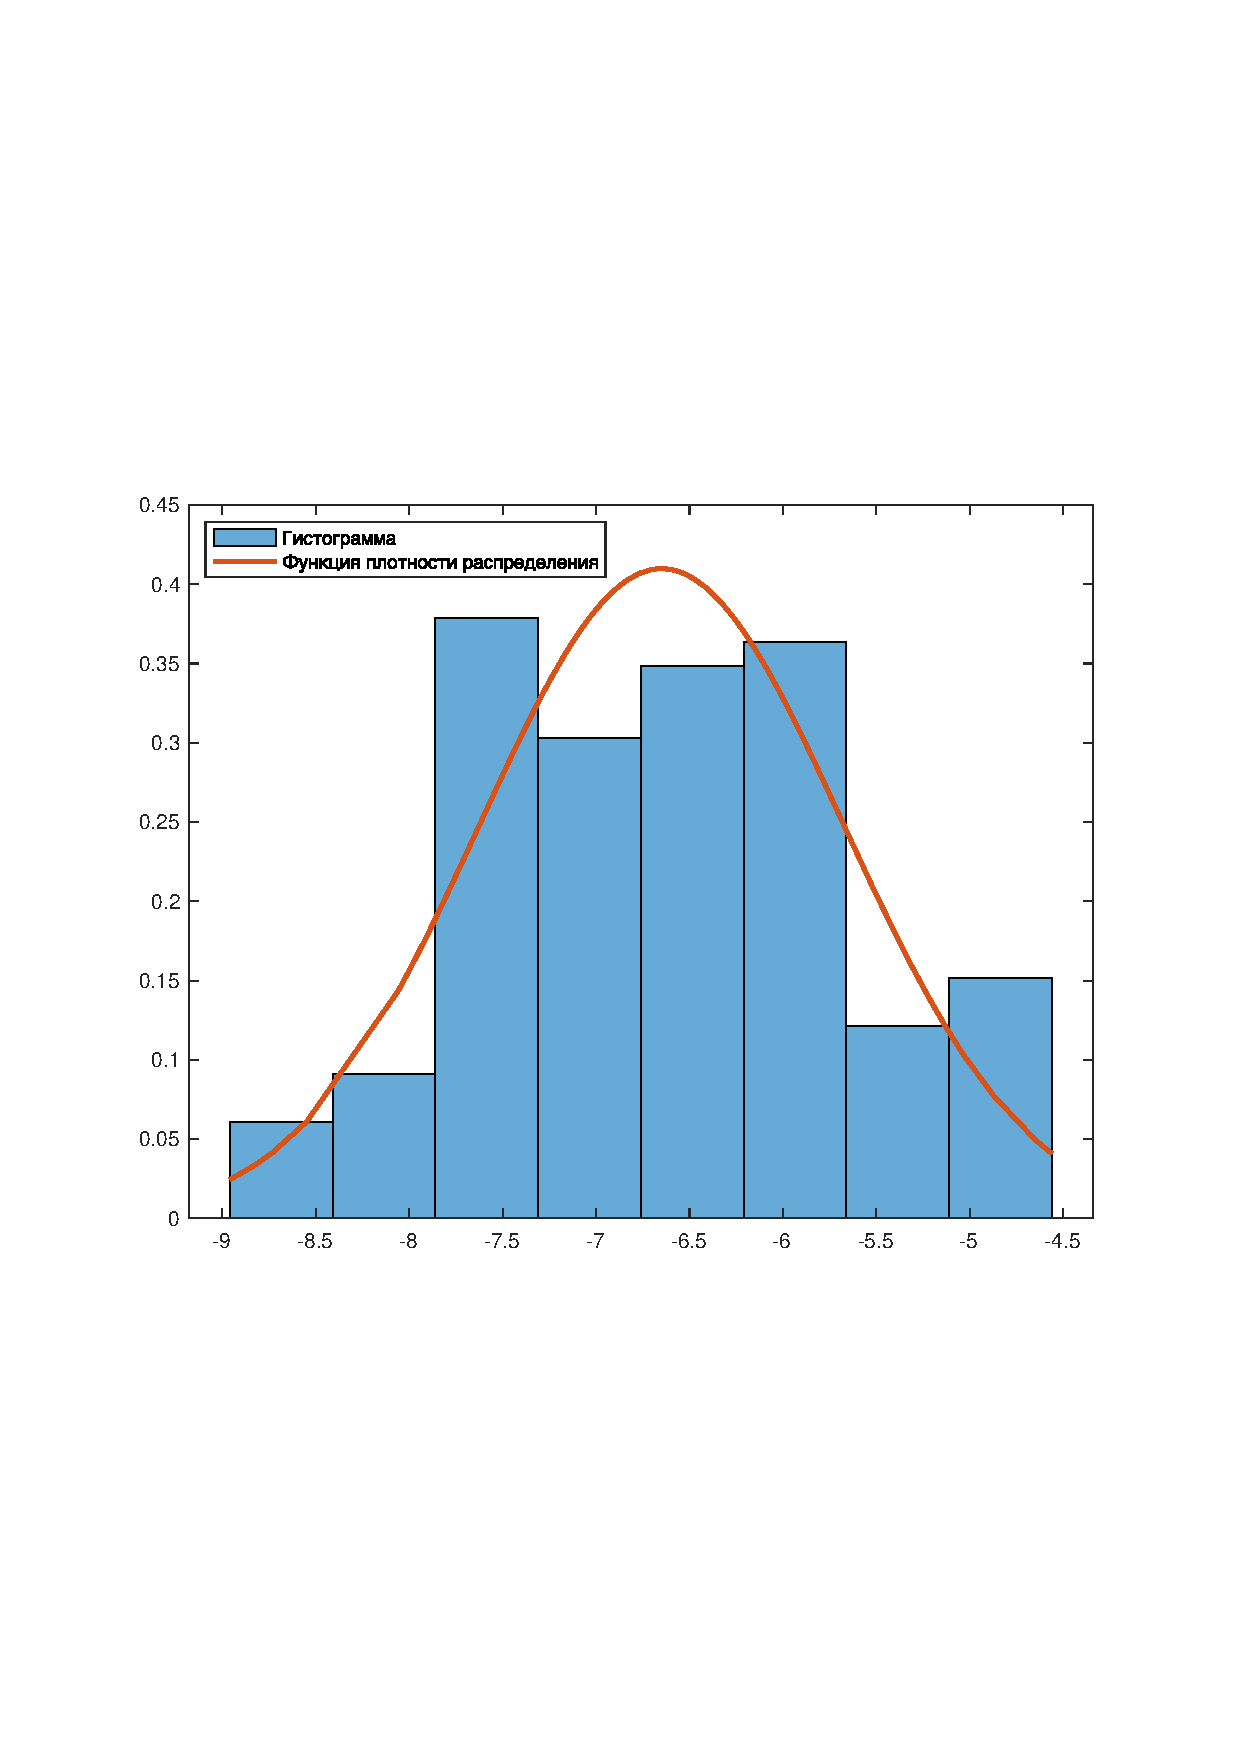
\includegraphics[trim=0.5cm 9cm 0.5cm 8cm]{img/histogram.pdf}
    \caption{Гистограмма}
\end{figure}

\begin{figure}[H]
    \centering
    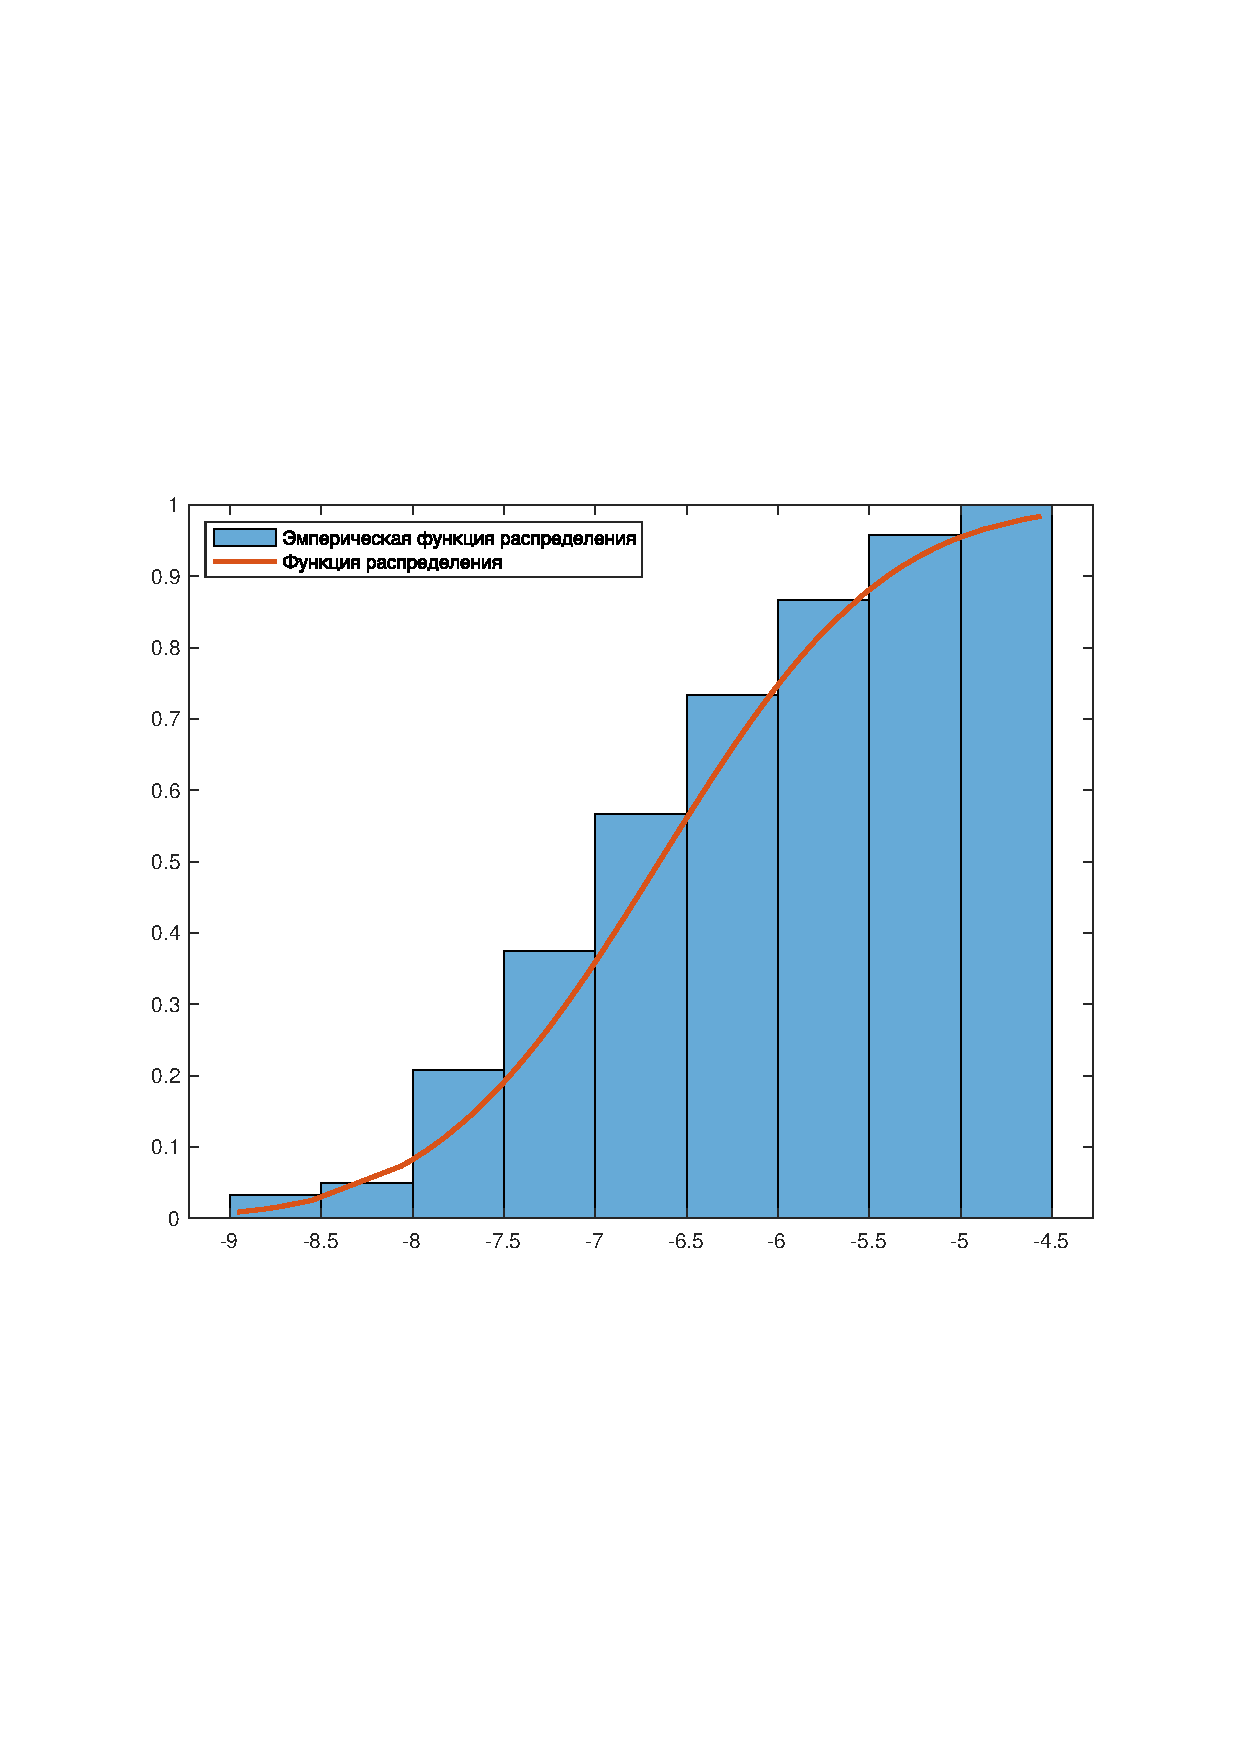
\includegraphics[trim=0.5cm 9cm 0.5cm 8cm]{img/emperical_graph.pdf}
    \caption{Эмперическая функция распределения}
\end{figure}
